\subsection{Hiện thực đổi món sau thanh toán}
\label{sec:exchange-implementation}
ExchangeService.quote/quoteIn tính báo giá từ dữ liệu backend; request kiểm quyền, trạng thái, yêu cầu chờ và key trước khi lưu báo giá. withdraw rút yêu cầu bằng trạng thái/version. decide thực hiện quyết định của quầy. Hàng đợi hỗ trợ lọc trạng thái, tìm kiếm và phân trang; frontend ExchangeWorkspace giữ giỏ đổi riêng, không trộn với lần mua thông thường.

\subsubsection{Một quyết định, một transaction}
decide khóa Order nguồn trước, đọc lại OrderExchange và kiểm version/REQUESTED. Khi duyệt, kiểm nguồn còn PAID và tiền đã áp dụng khớp; dùng quotedLines để giữ thành tiền đã chấp nhận. Tiếp theo khóa tập hợp nguyên liệu cũ và mới theo id tăng dần, hoàn snapshot cũ, reserve lựa chọn mới theo size/topping, tạo Order thay thế và snapshot, chuyển credit rồi đóng Order nguồn. Cuối cùng cập nhật quyết định, tăng version và commit. Thiếu nguyên liệu mới hoặc lỗi bất kỳ làm rollback cả bước hoàn cũ.

\subsubsection{Tranh chấp với pha chế và thao tác quầy}
Luồng bắt đầu pha và quyết định đổi cùng khóa Order. API bắt đầu pha kiểm yêu cầu REQUESTED; API duyệt kiểm nguồn PAID. Vì vậy thao tác dựa trên trạng thái cũ bị chặn sau khi trạng thái đã thay đổi. UPDATE yêu cầu có điều kiện id/version/status và kiểm count=1 bảo vệ trước thao tác đã cũ; version tăng sau khi duyệt, từ chối hoặc rút. Thông báo UI phát sau commit.

\subsubsection{Bảo toàn tiền đã chuyển}
Đơn thay thế có credit không đi qua tự hủy/hết hạn thông thường của đơn chưa từng trả tiền. Các thao tác giữ/hoàn tài nguyên tái sử dụng cơ chế mục~\ref{sec:inventory-implementation}; thu chênh lệch tái sử dụng VNPay mục~\ref{sec:vnpay-implementation}. Không cộng credit thành một Payment mới, vì việc đó sẽ làm sai thống kê dòng tiền và có thể cộng điểm trùng.

\begin{figure}[htbp]\centering
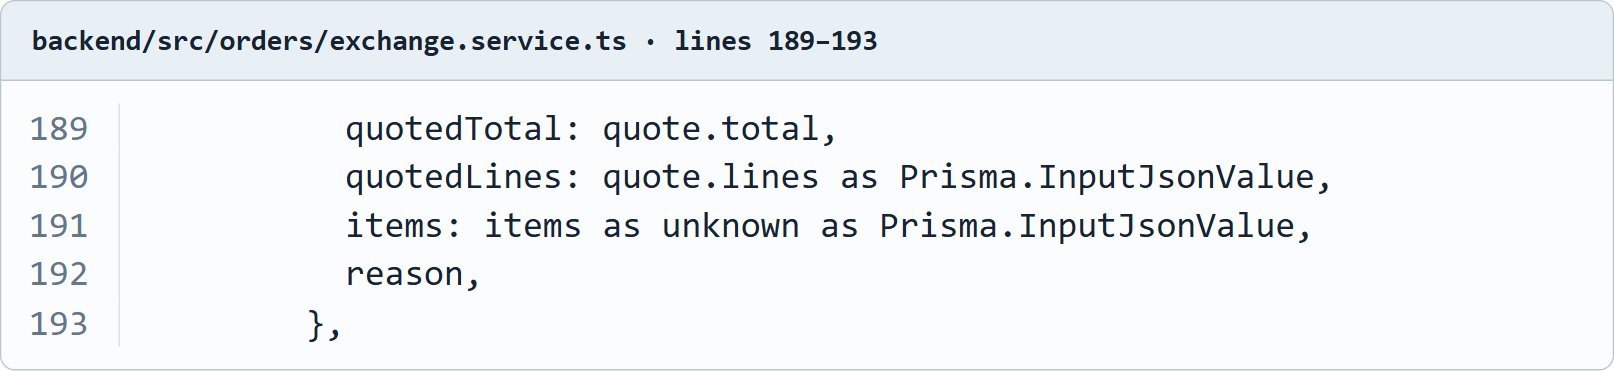
\includegraphics[width=.94\linewidth,height=.25\textheight,keepaspectratio]{assets/exchange/code-quote.png}
\caption{request lưu báo giá và nội dung đã được khách xác nhận}
\vspace{3mm}
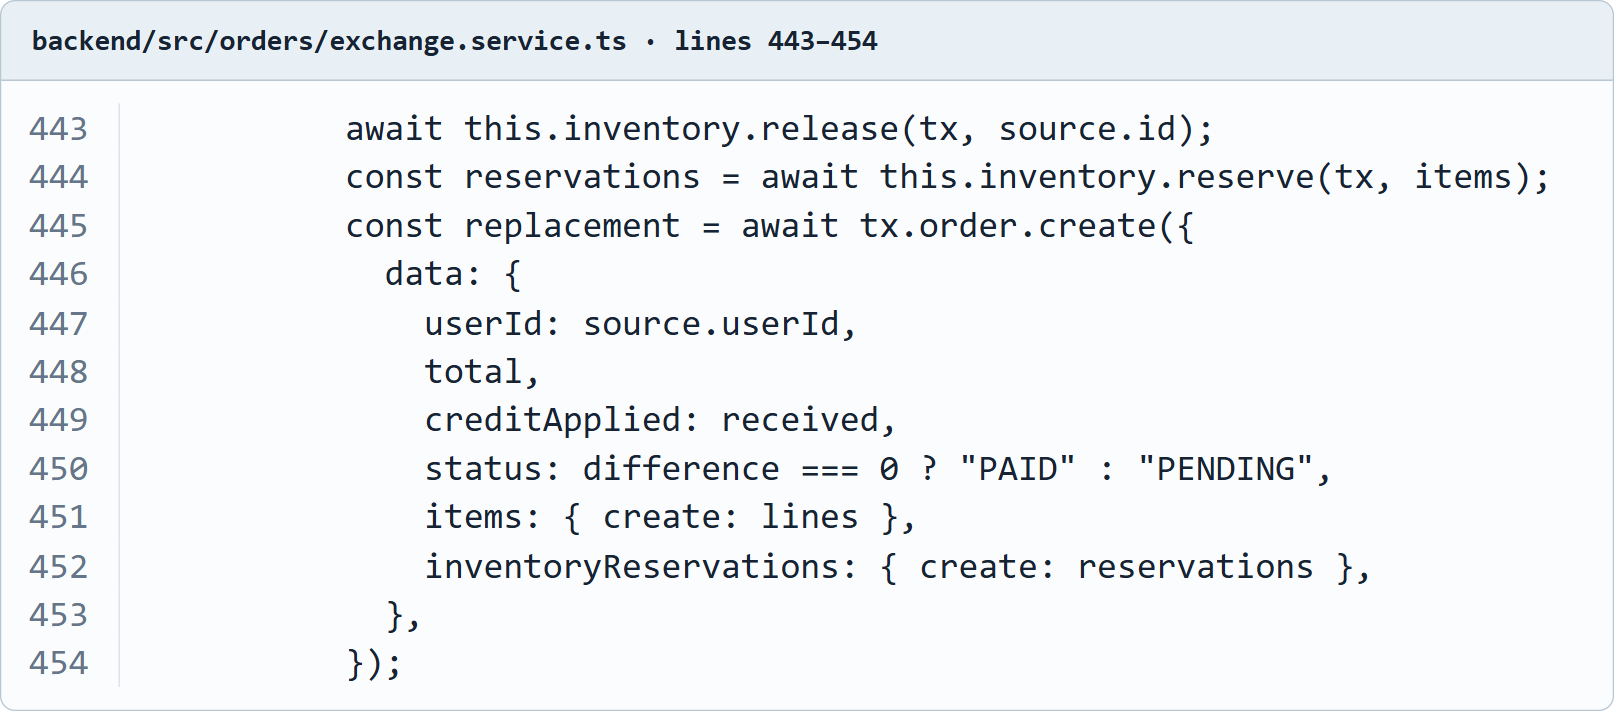
\includegraphics[width=.94\linewidth,height=.26\textheight,keepaspectratio]{assets/exchange/code-replacement.png}
\caption{Hoàn snapshot cũ, giữ lựa chọn mới và tạo đơn chuyển credit trong transaction}
\vspace{3mm}
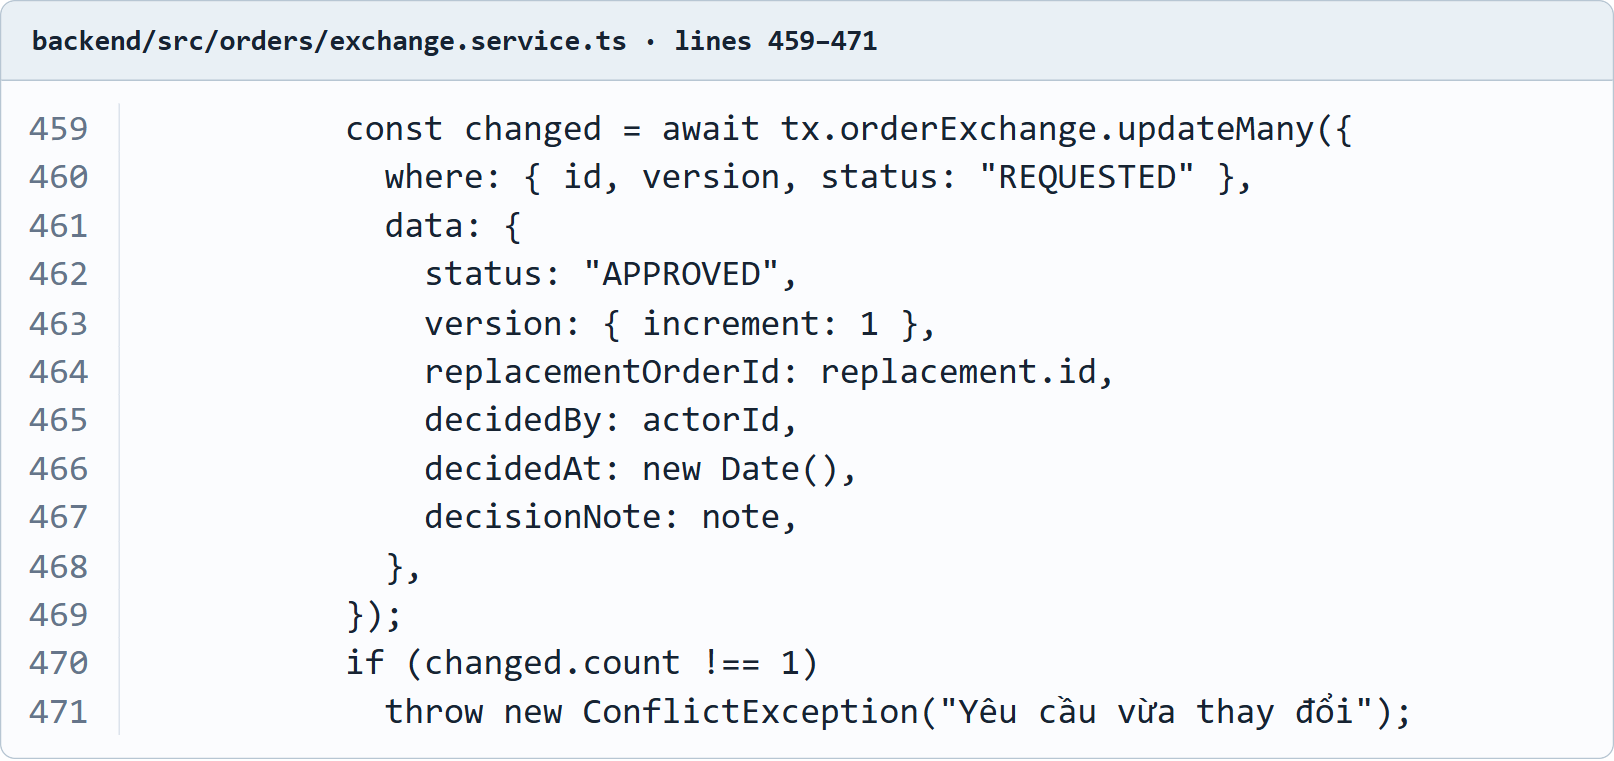
\includegraphics[width=.94\linewidth,height=.25\textheight,keepaspectratio]{assets/exchange/code-version.png}
\caption{Quyết định cập nhật có điều kiện theo version và trạng thái REQUESTED}
\end{figure}
